\section{Introduction}

Every electronic device requires the use of a timing system (usually referred as clock) that sets the reference for the operation of the device.
This timing system is implemented through the use of various electronic components such as clock source, phase comparator, frequency dividers\dots.

The aim of this project is to investigate the state of the art of clock sources technologies, with a focus on the most recent advancements in the field and their potential applications.
In particular, the project will focus on the following topics:

\begin{itemize}
    \item \semph{Crystal oscillators} (optional) : electric oscillator type circuit that uses a piezoelectric resonator, a crystal, as its frequency-determining element (\href{https://en.wikipedia.org/wiki/Crystal_oscillator#Terminology}{Wikipedia definition}).
    \item \semph{\acrshort{mems} resonators} (main focus) : small electromechanical structures that vibrate at high frequencies (\href{https://en.wikipedia.org/wiki/Microelectromechanical_system_oscillator#Resonators}{Wikipedia definition}).
    \item \semph{\acrshort{mems} Atomic Clocks} (time permitting): the combination of a \acrshort{mems} system fabrication with atomic clocks for small, cheap, low-power devices \cite{KNAPPE2008571}.
\end{itemize}

\begin{figure}[H]
    \begin{minipage}[b]{0.30\textwidth}
        \centering
        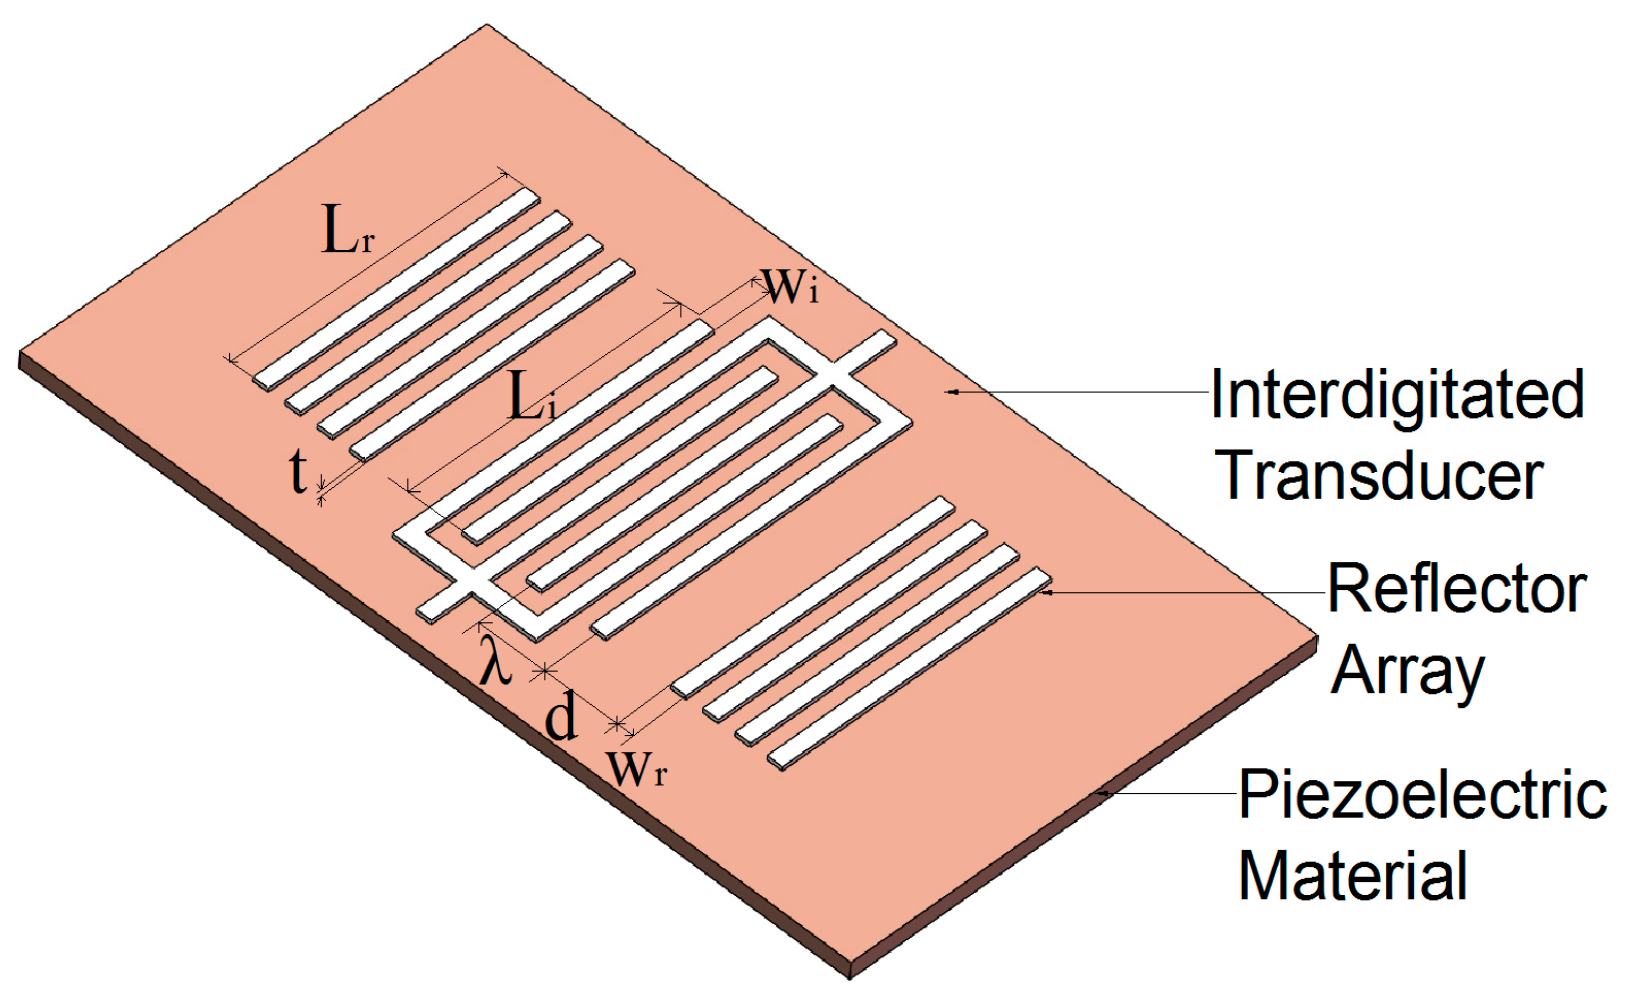
\includegraphics[width=\textwidth]{img/SAW_oscillator}
        \caption{Schematic diagram of SAW resonator \cite{mi10060349}}
    \end{minipage}
    \hfill
    \begin{minipage}[b]{0.30\textwidth}
        \centering
        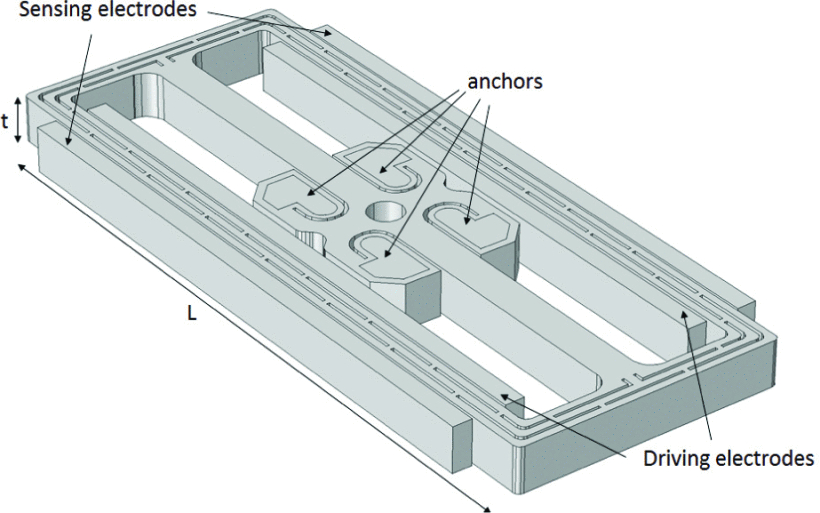
\includegraphics[width=\textwidth]{img/MEMS_resonators}
        \caption{MEMS oscillator \cite{KNAPPE2008571}}
    \end{minipage}
    \hfill
    \begin{minipage}[b]{0.30\textwidth}
        \centering
        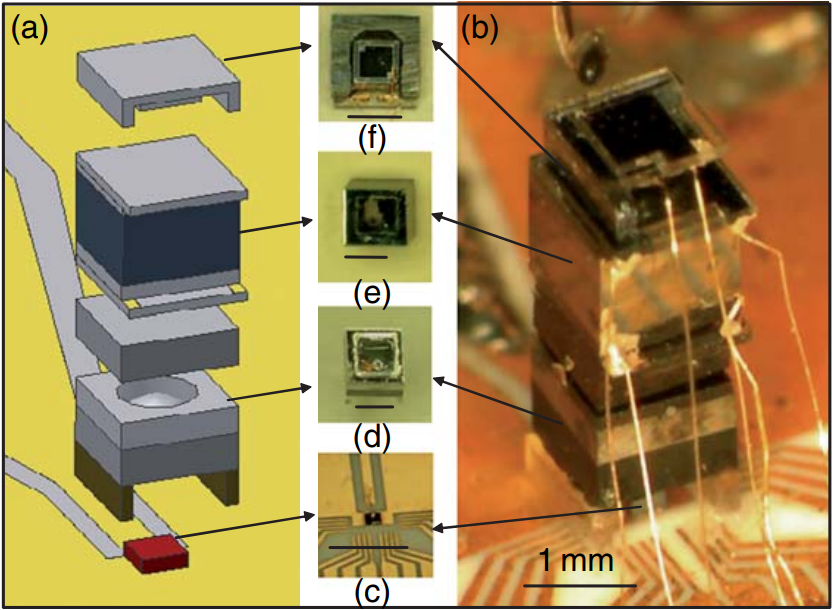
\includegraphics[width=\textwidth]{img/atomic_clock_chip_scale}
        \caption{Chip-scale atomic clock (CSAC) \cite{8956703}}
    \end{minipage}
\end{figure}

Topics are mostly indicative and will be refined during the project development also based on professor's feedback, affinity with the course subjects, and personal interests.
